\begin{figure}[htbp]
\centering
\makebox[\textwidth][c]{%
\begin{minipage}{18.5cm}\centering
\begin{minipage}[t]{0.326\textwidth}\centering
{\fontsize{10}{12}\selectfont\bfseries Cell2}\\[-0.1em]
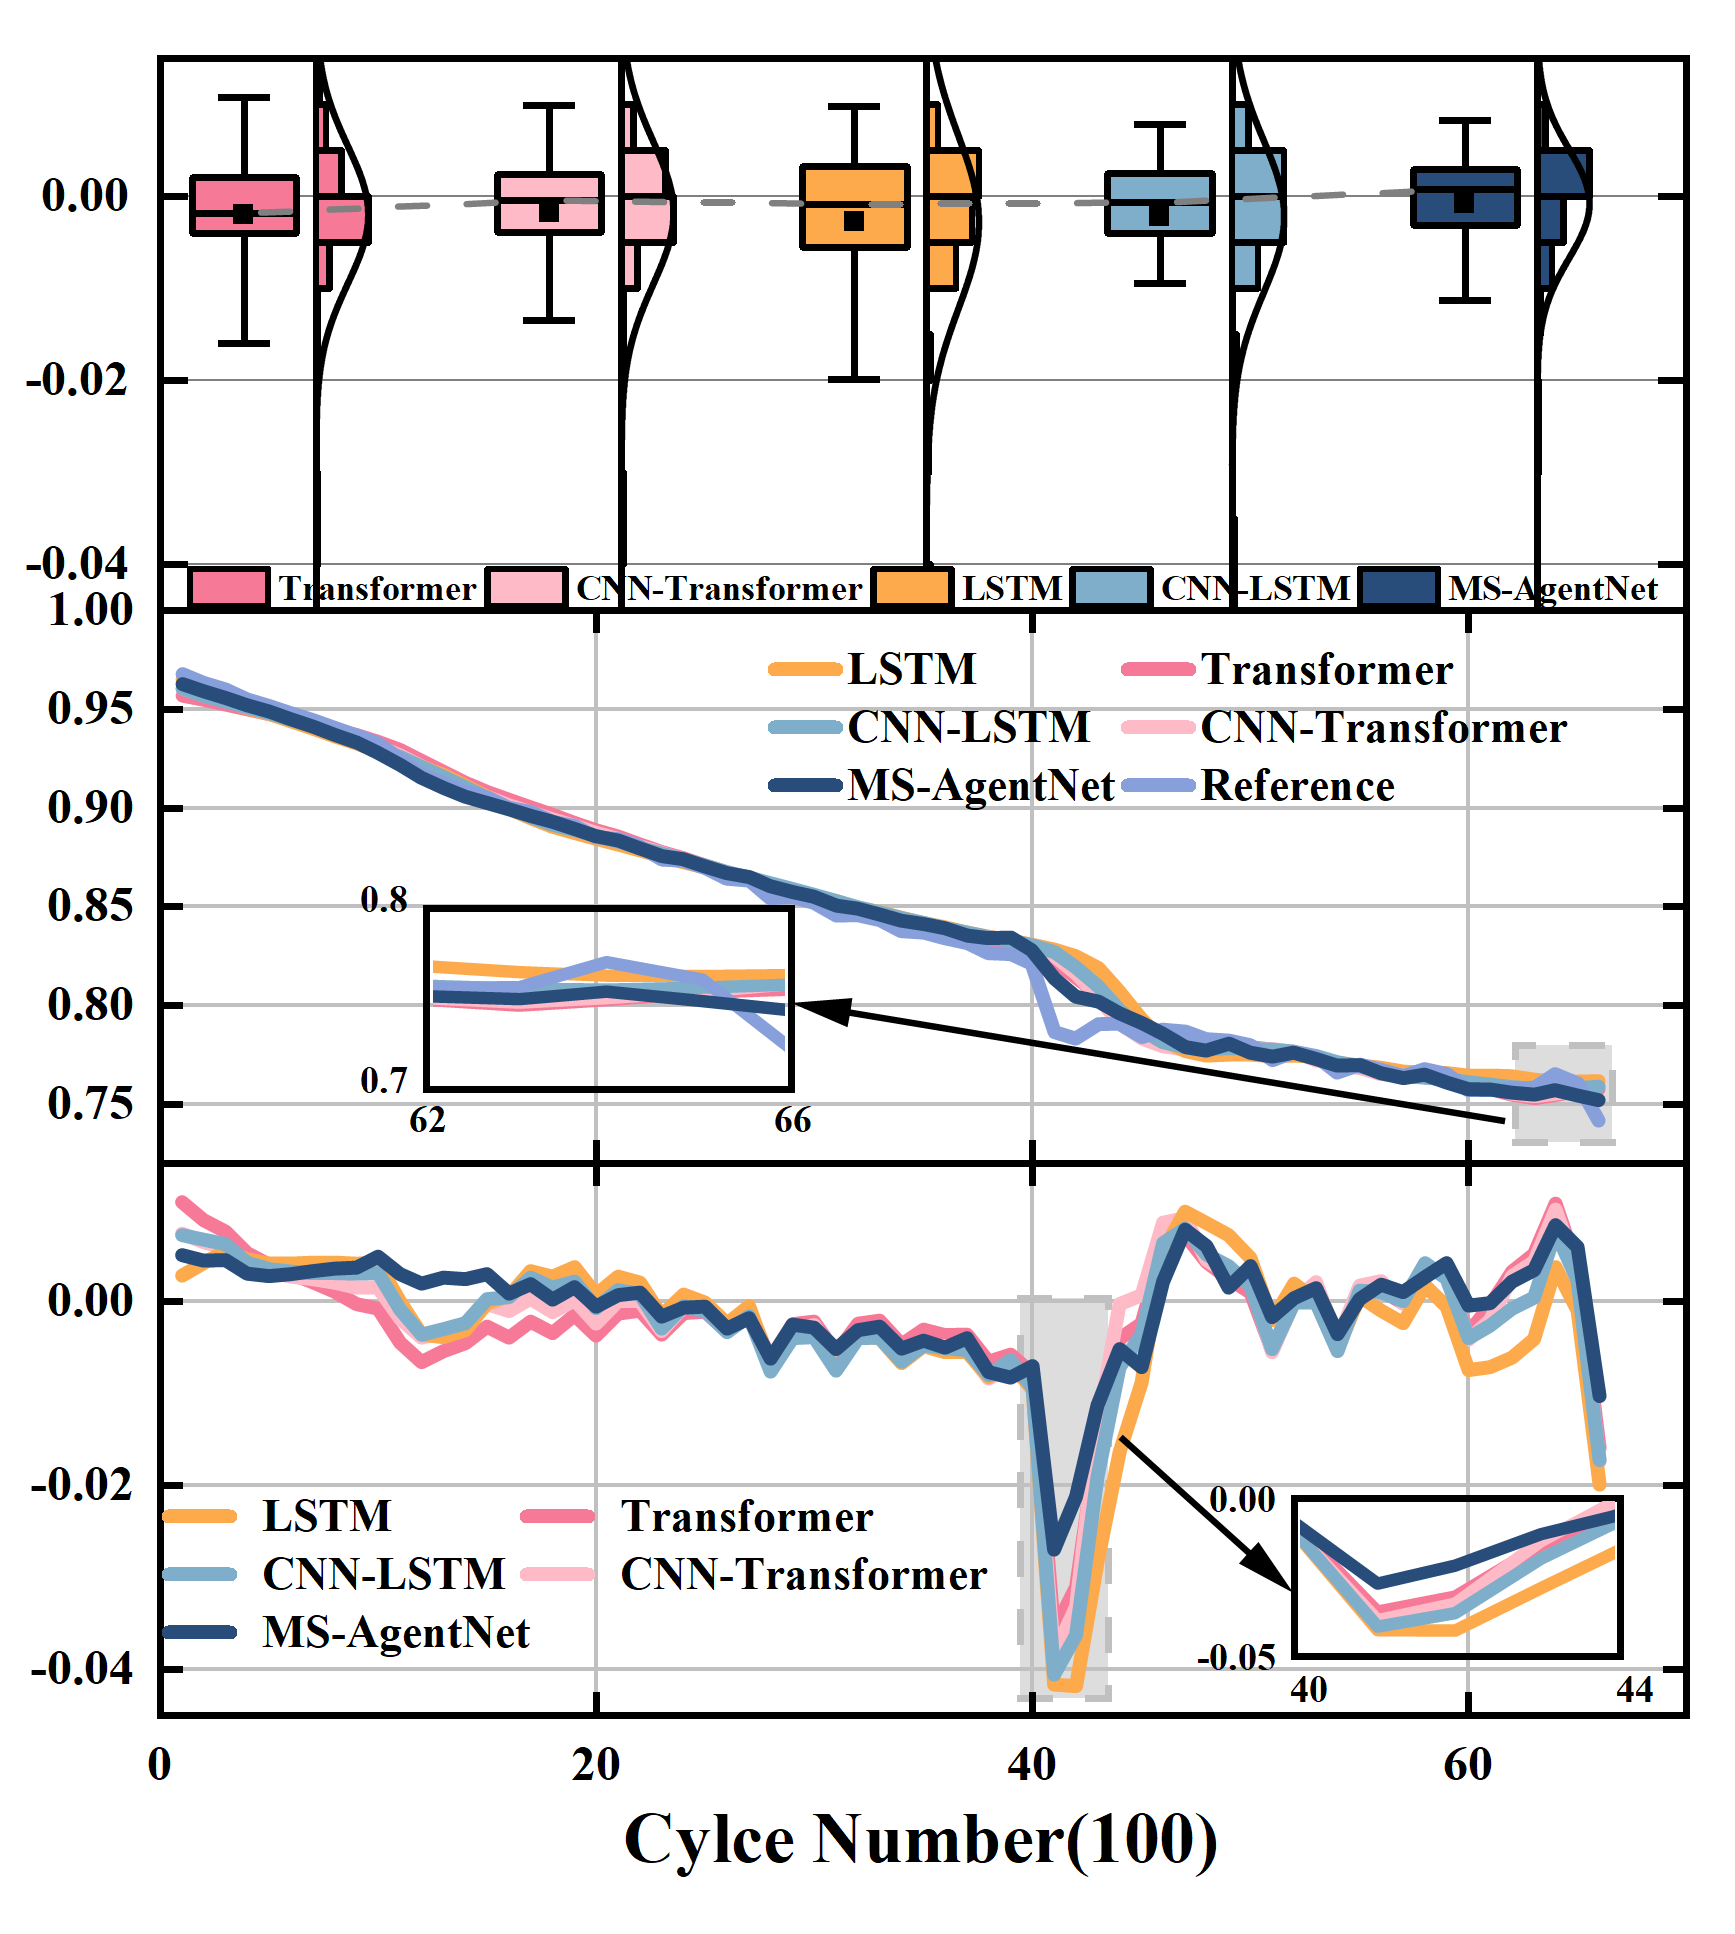
\includegraphics[width=\linewidth]{figures/Oxford/cell2.png}
\end{minipage}%
\hspace{0.01\textwidth}%
\begin{minipage}[t]{0.326\textwidth}\centering
{\fontsize{10}{12}\selectfont\bfseries Cell3}\\[-0.1em]
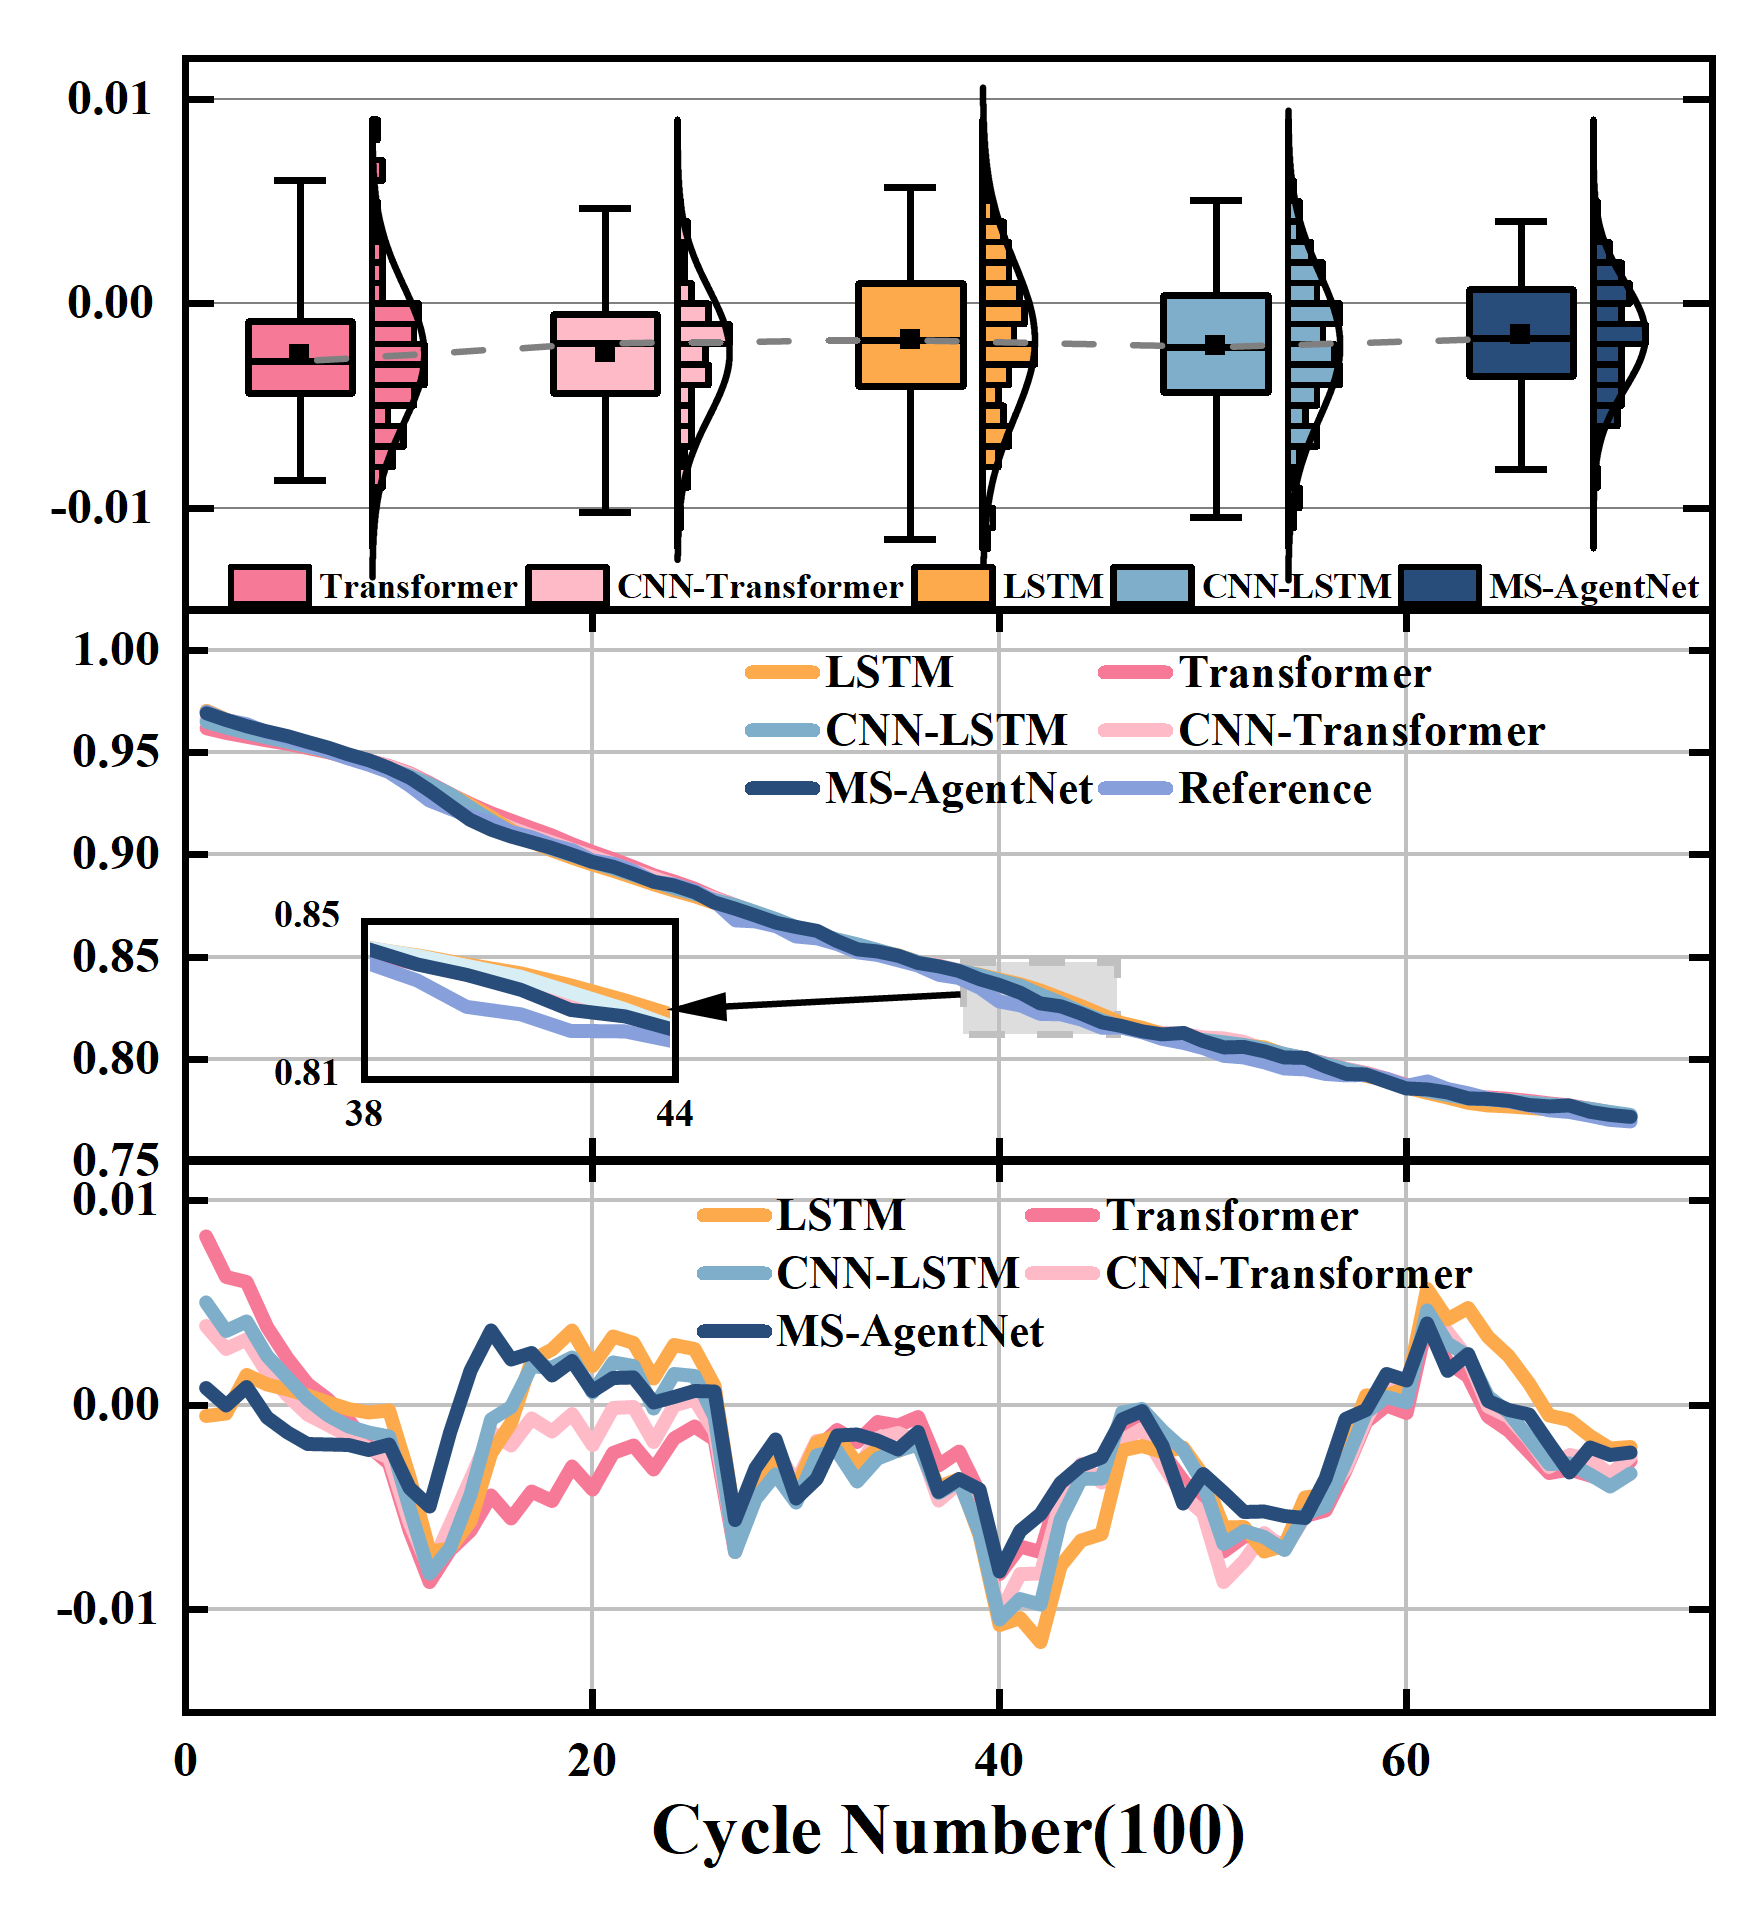
\includegraphics[width=\linewidth]{figures/Oxford/cell3.png}
\end{minipage}%
\\[0.7em]
\begin{minipage}[t]{0.326\textwidth}\centering
{\fontsize{10}{12}\selectfont\bfseries Cell4}\\[-0.1em]
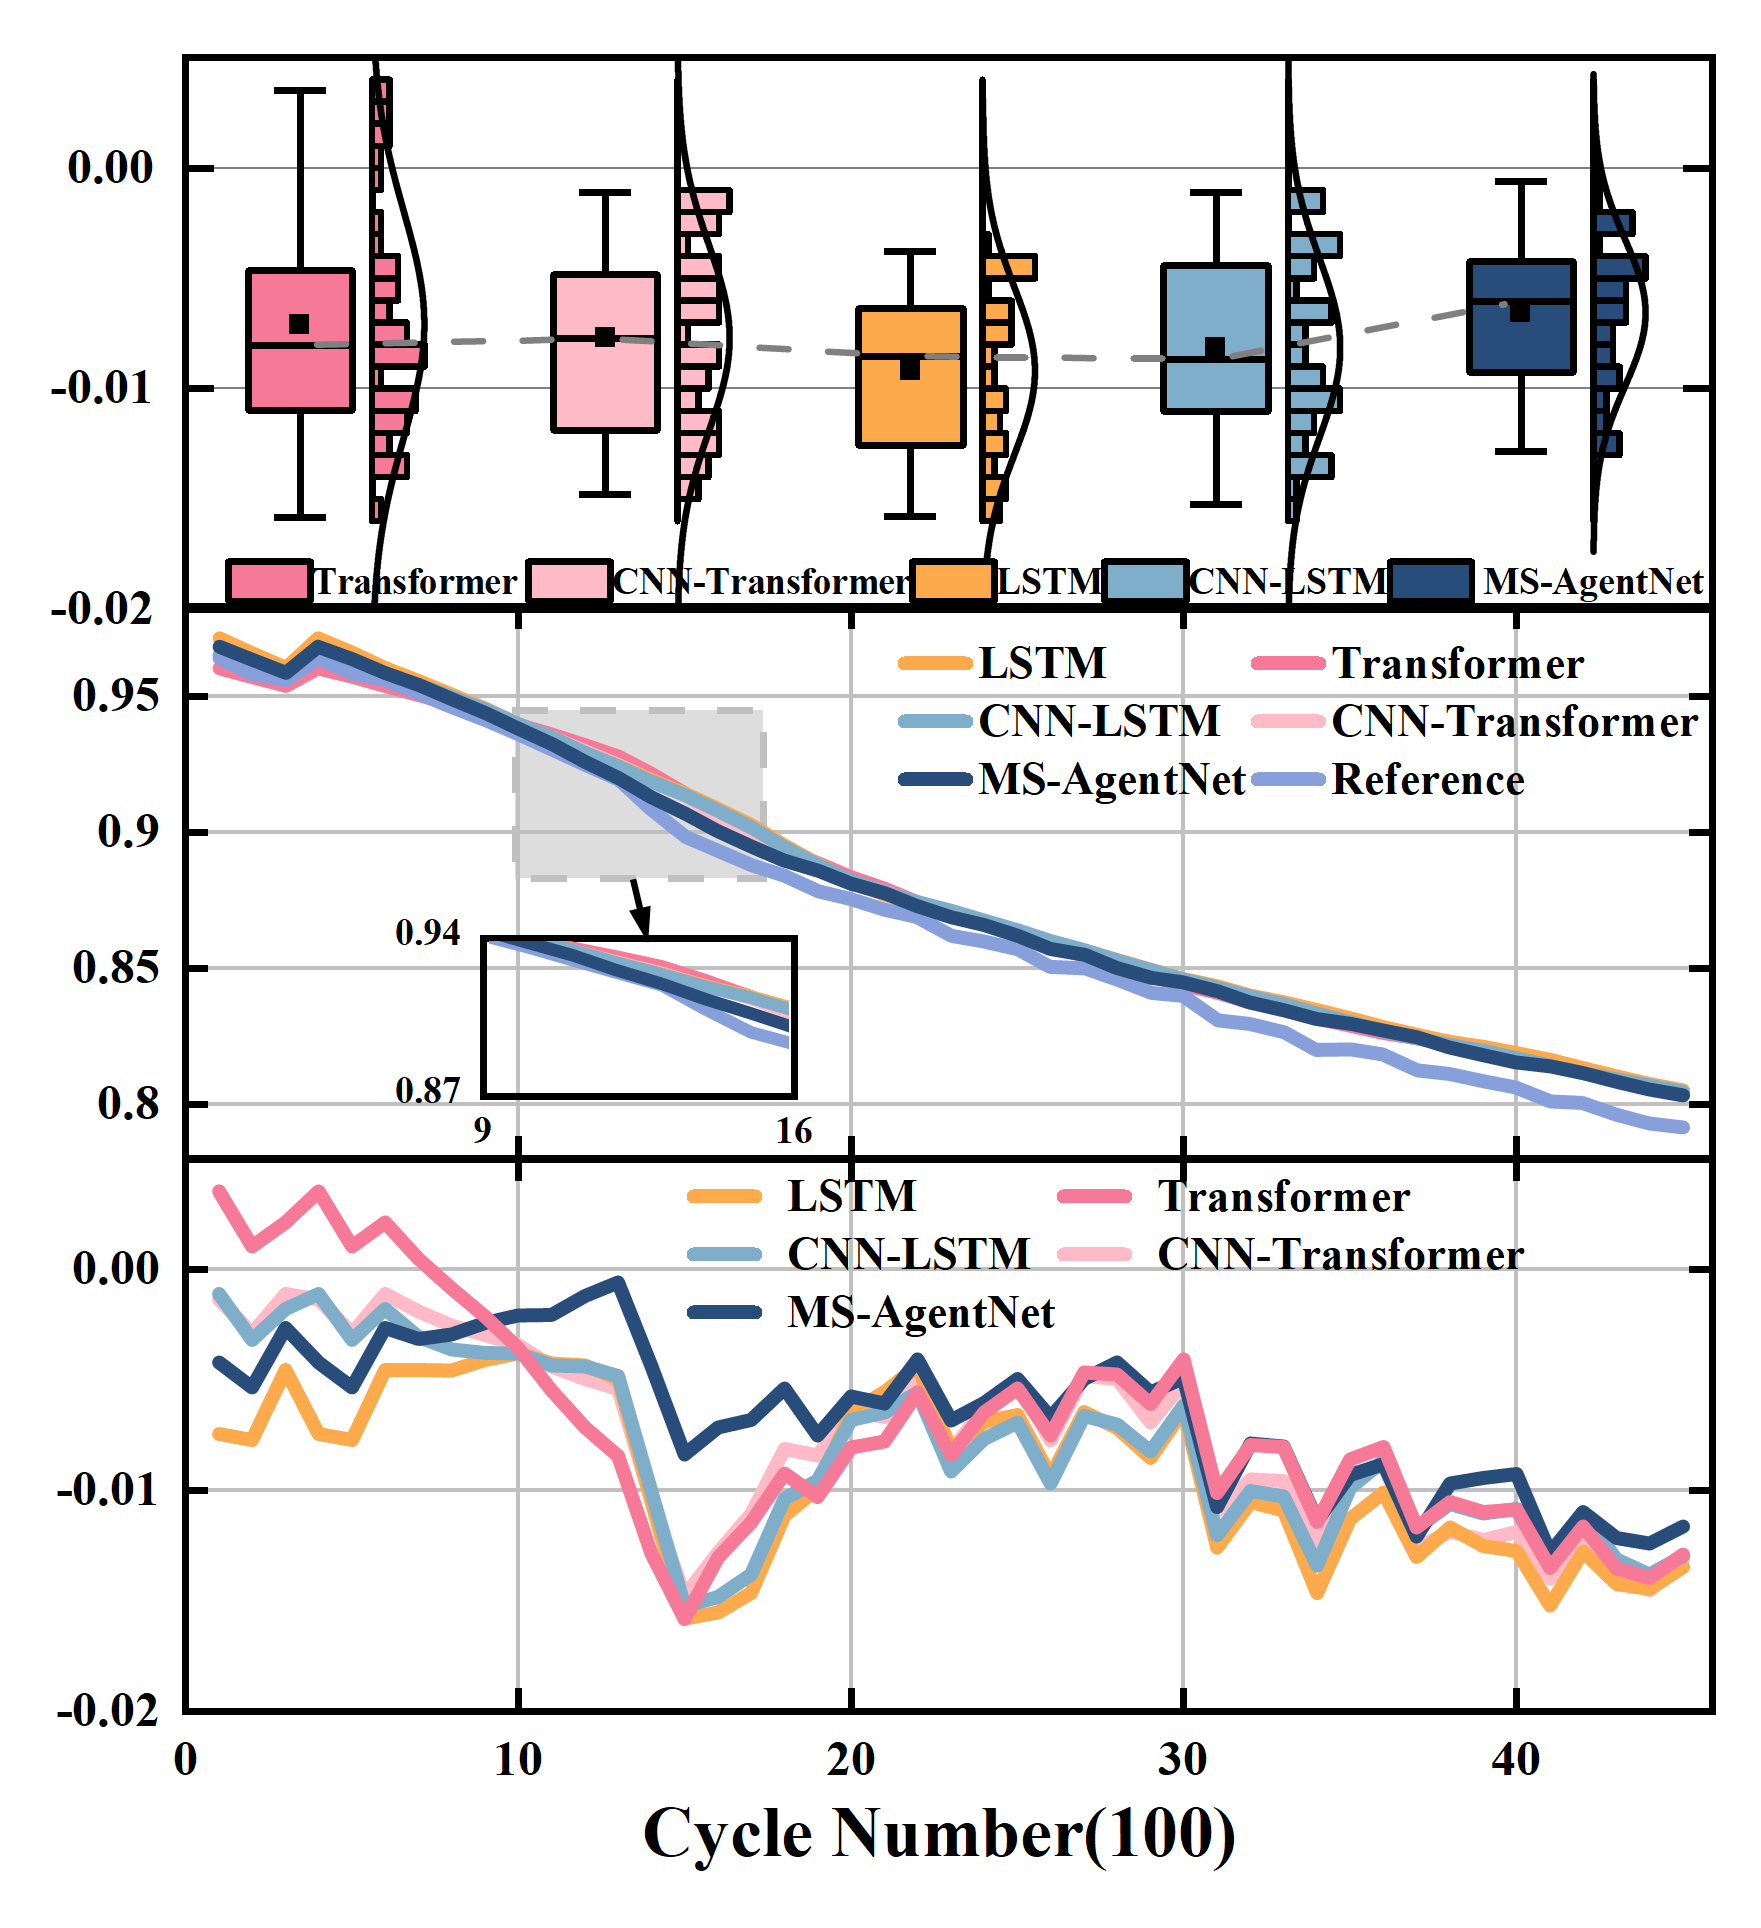
\includegraphics[width=\linewidth]{figures/Oxford/cell4.png}
\end{minipage}%
\hspace{0.01\textwidth}%
\begin{minipage}[t]{0.326\textwidth}\centering
{\fontsize{10}{12}\selectfont\bfseries Cell5}\\[-0.1em]
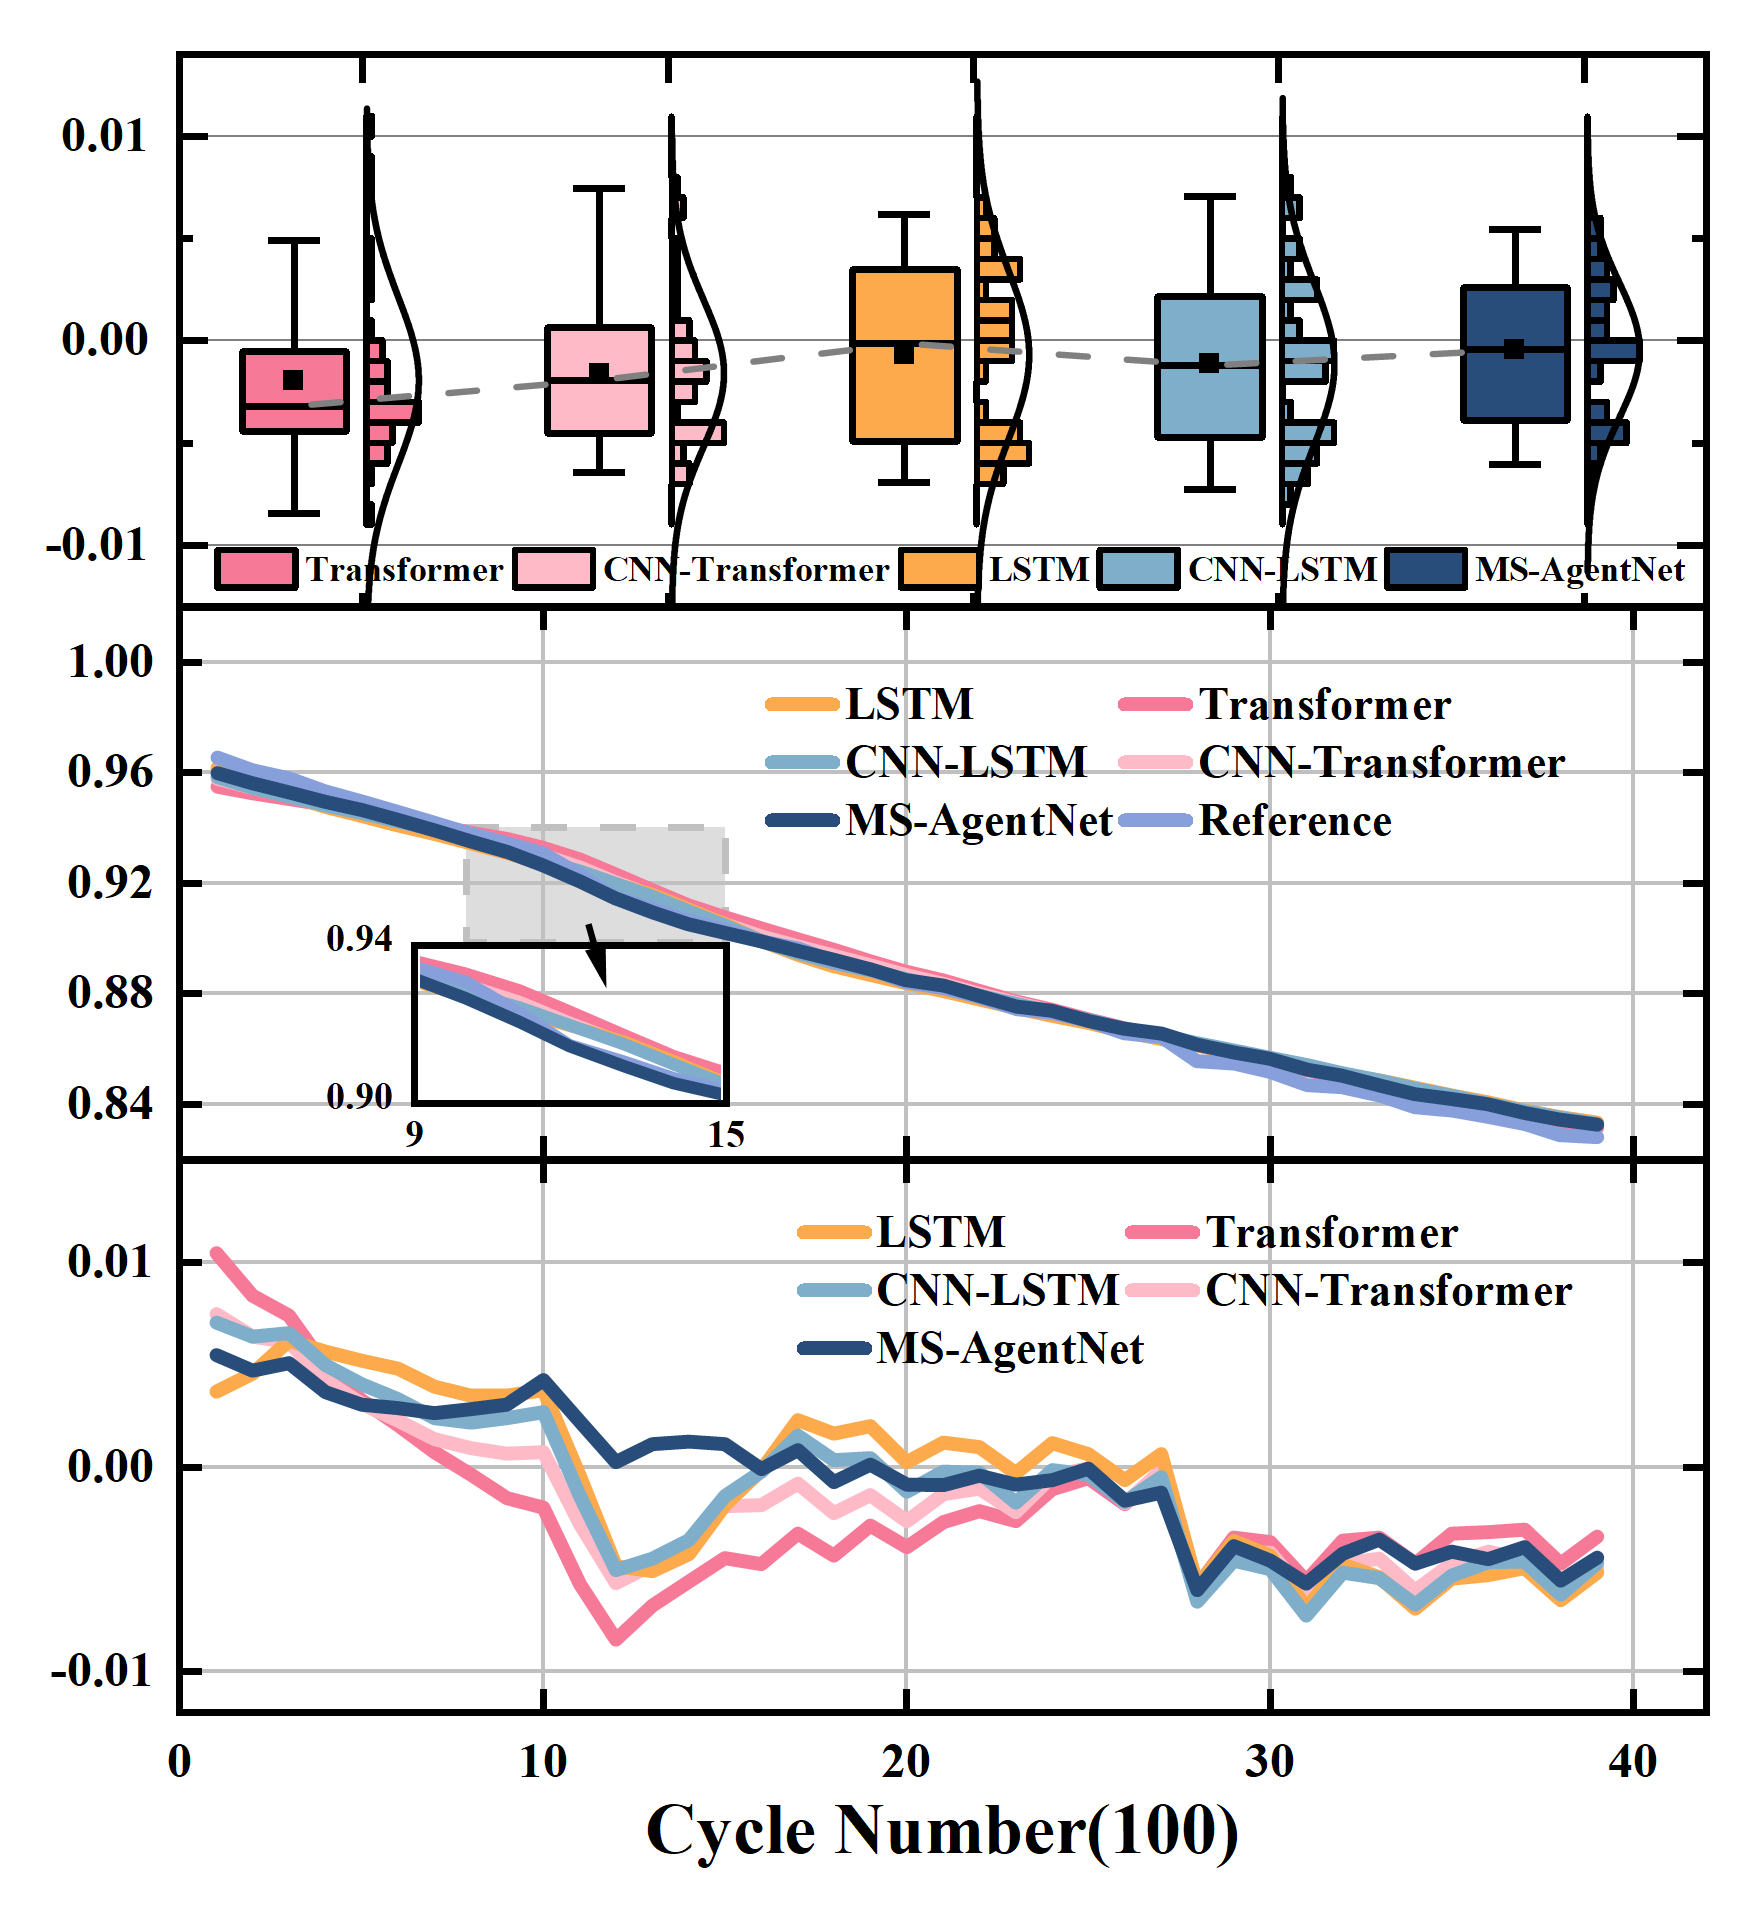
\includegraphics[width=\linewidth]{figures/Oxford/cell5.png}
\end{minipage}%
\hspace{0.01\textwidth}%
\begin{minipage}[t]{0.326\textwidth}\centering
{\fontsize{10}{12}\selectfont\bfseries Cell6}\\[-0.1em]
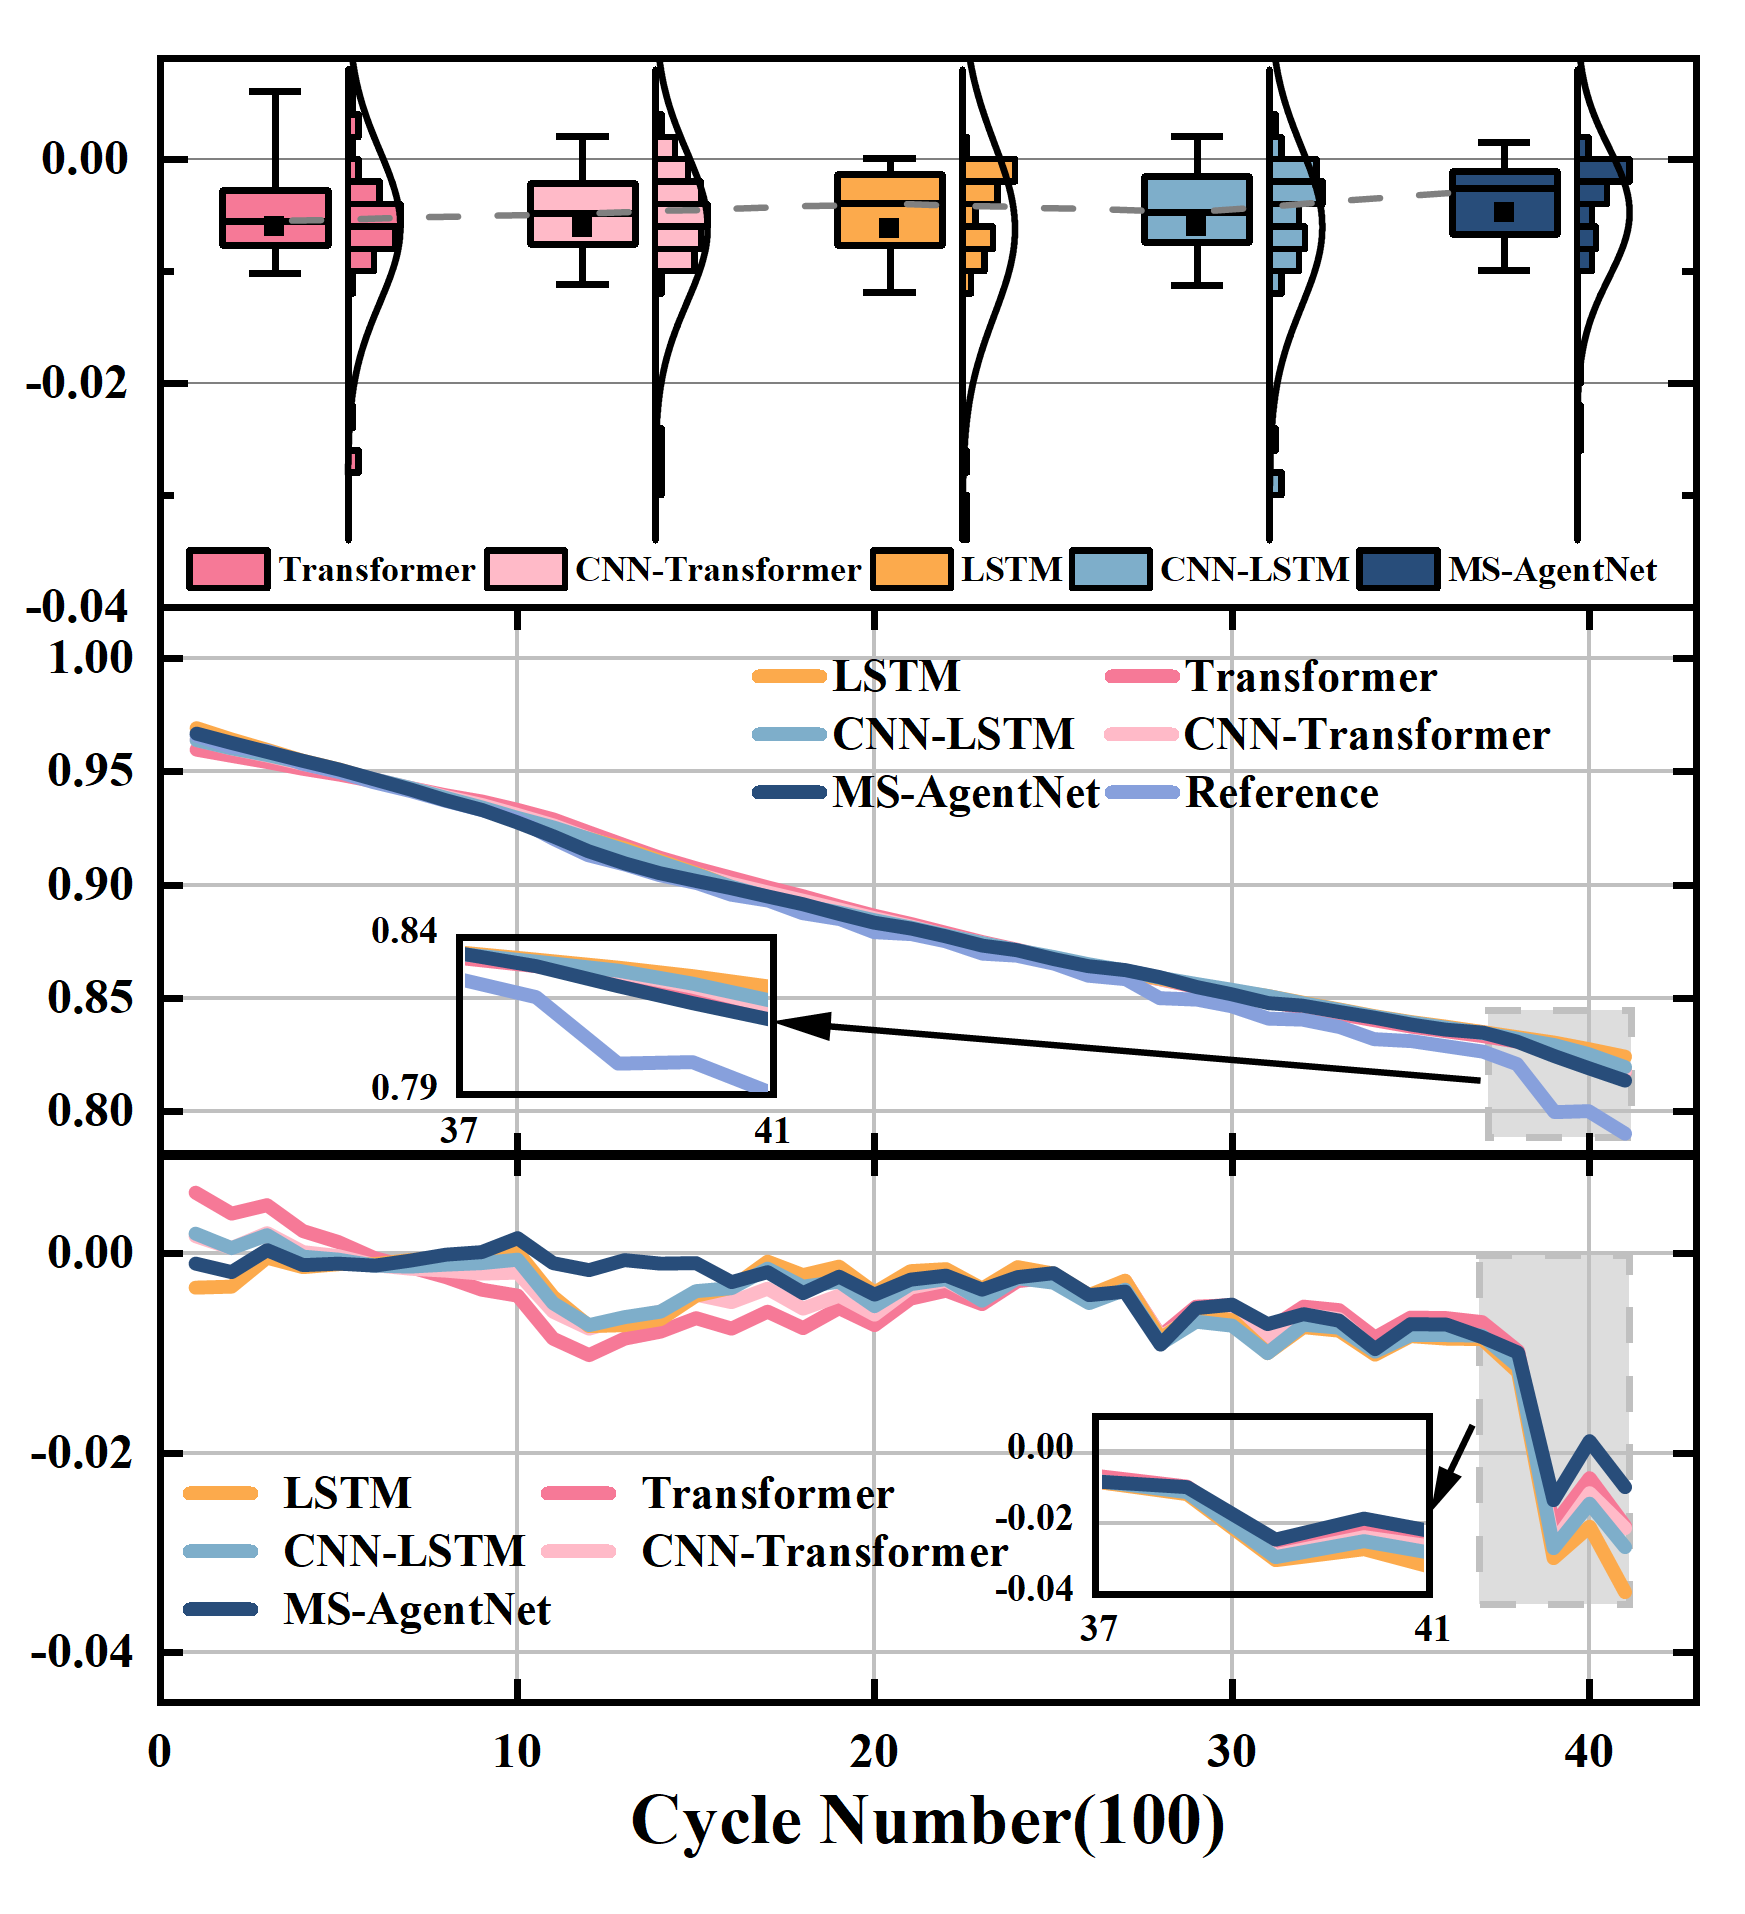
\includegraphics[width=\linewidth]{figures/Oxford/cell6.png}
\end{minipage}%
\\[0.7em]
\begin{minipage}[t]{0.326\textwidth}\centering
{\fontsize{10}{12}\selectfont\bfseries Cell7}\\[-0.1em]
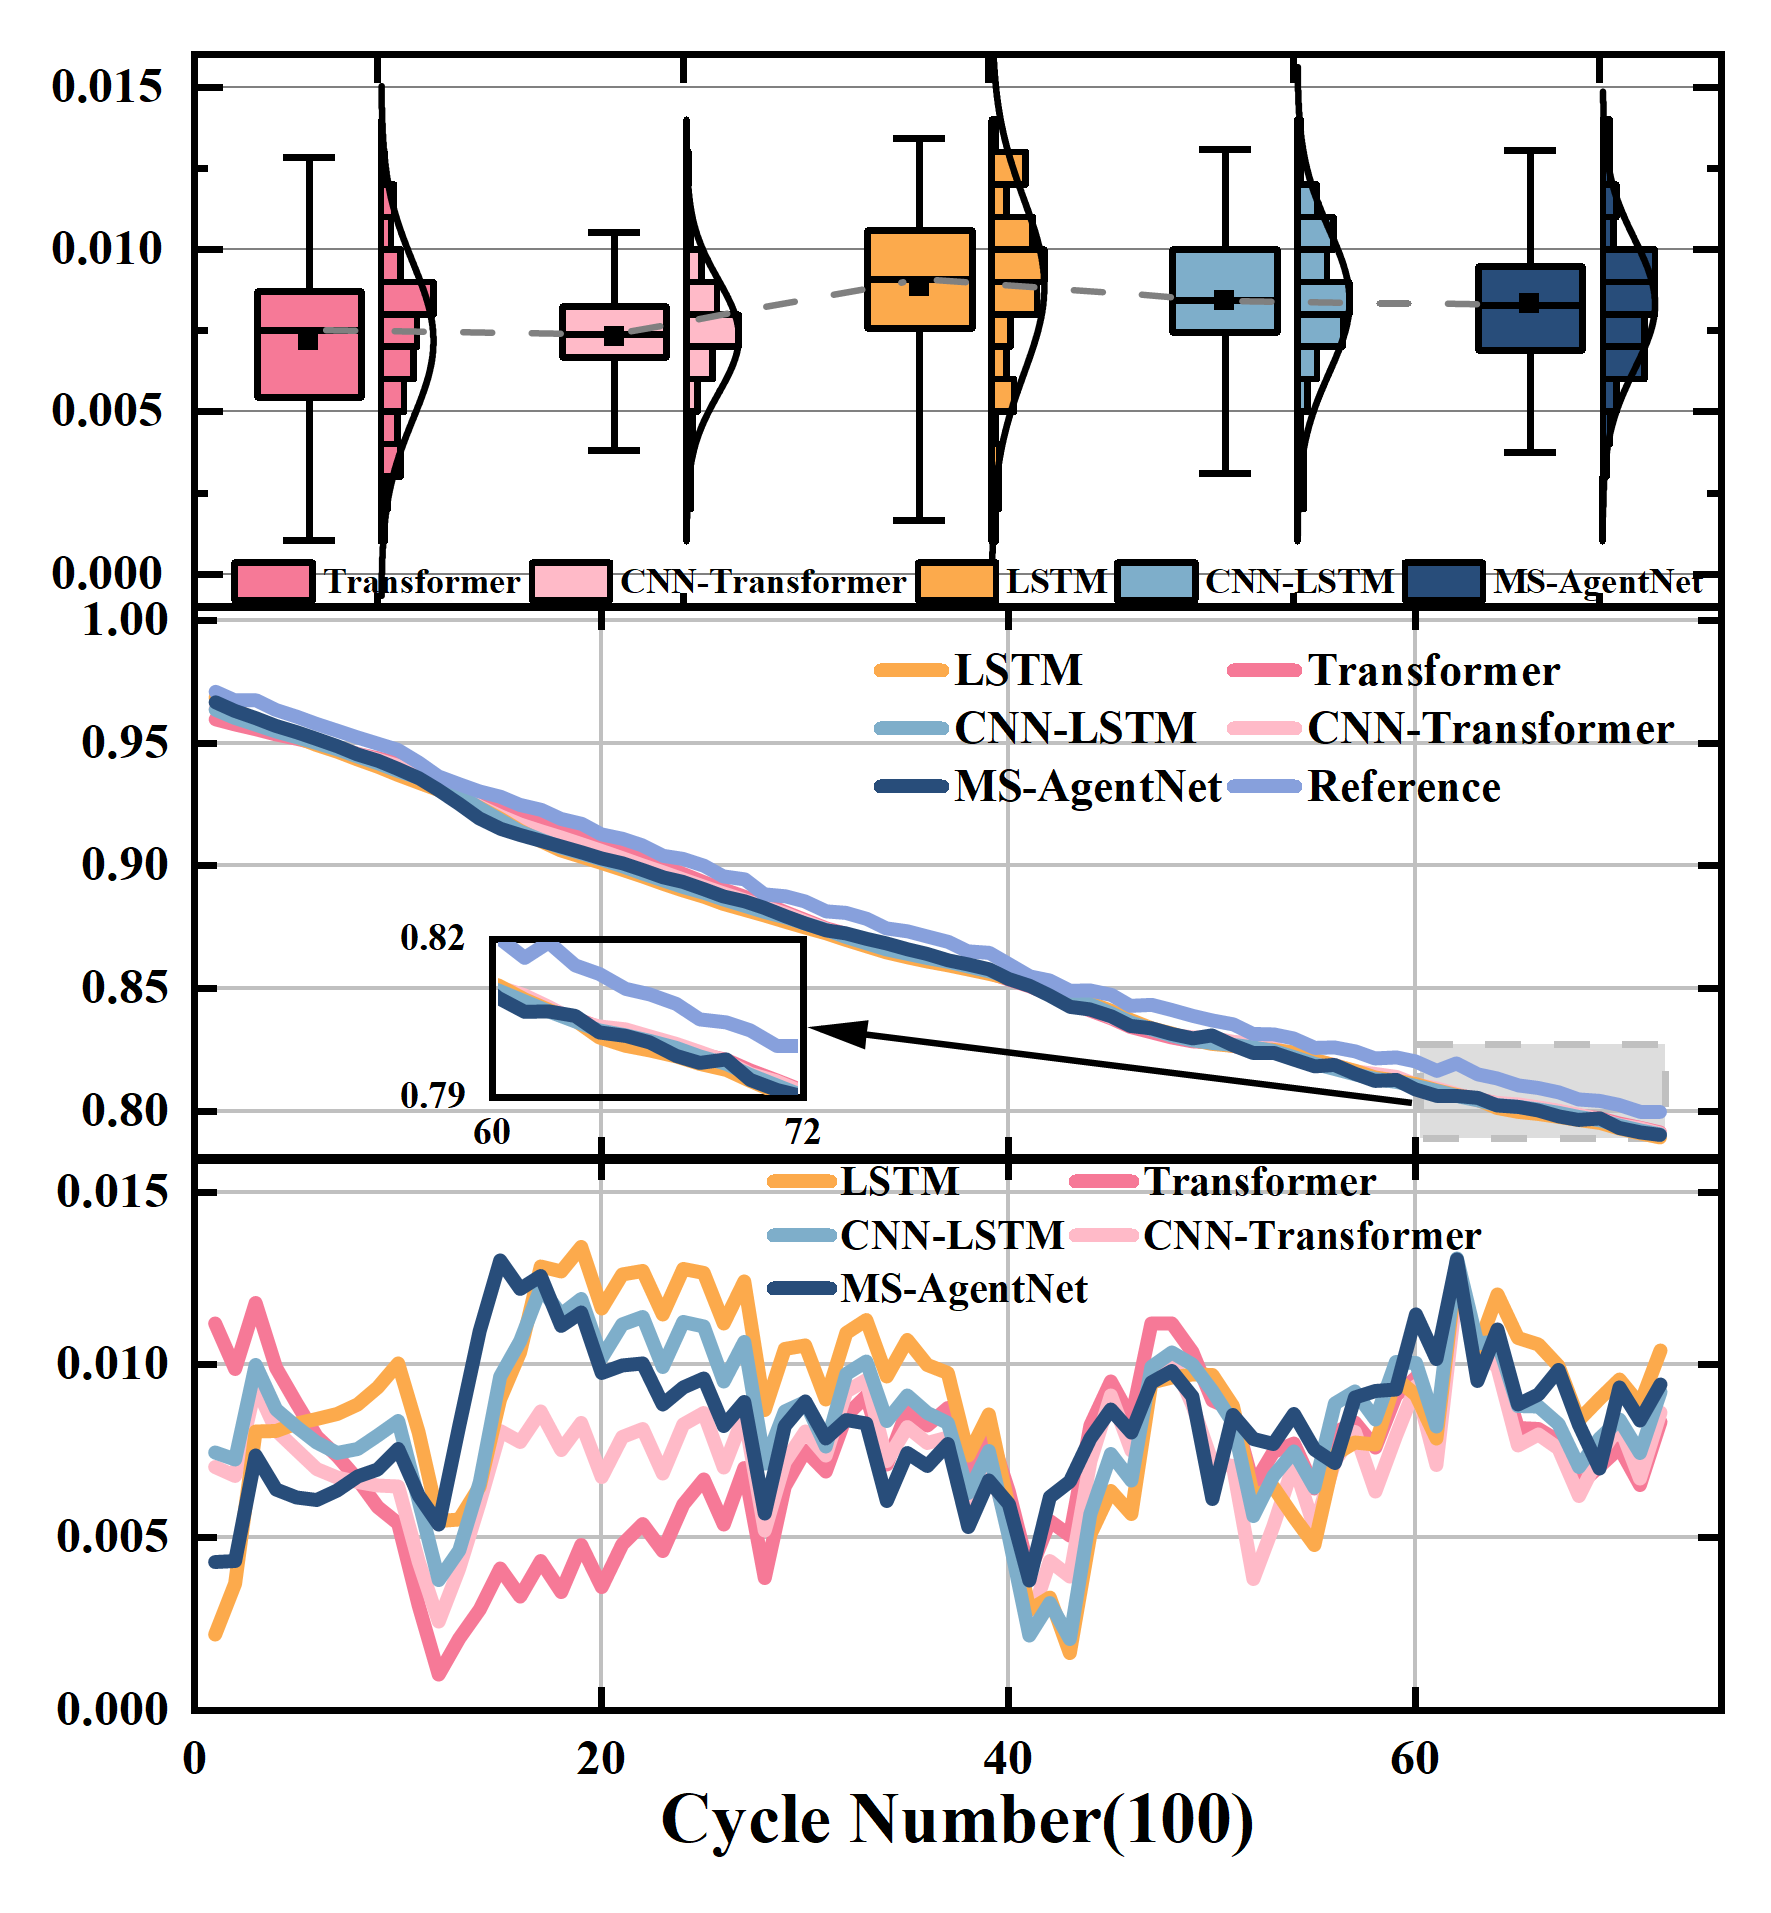
\includegraphics[width=\linewidth]{figures/Oxford/cell7.png}
\end{minipage}%
\hspace{0.01\textwidth}%
\begin{minipage}[t]{0.326\textwidth}\centering
{\fontsize{10}{12}\selectfont\bfseries Cell8}\\[-0.1em]
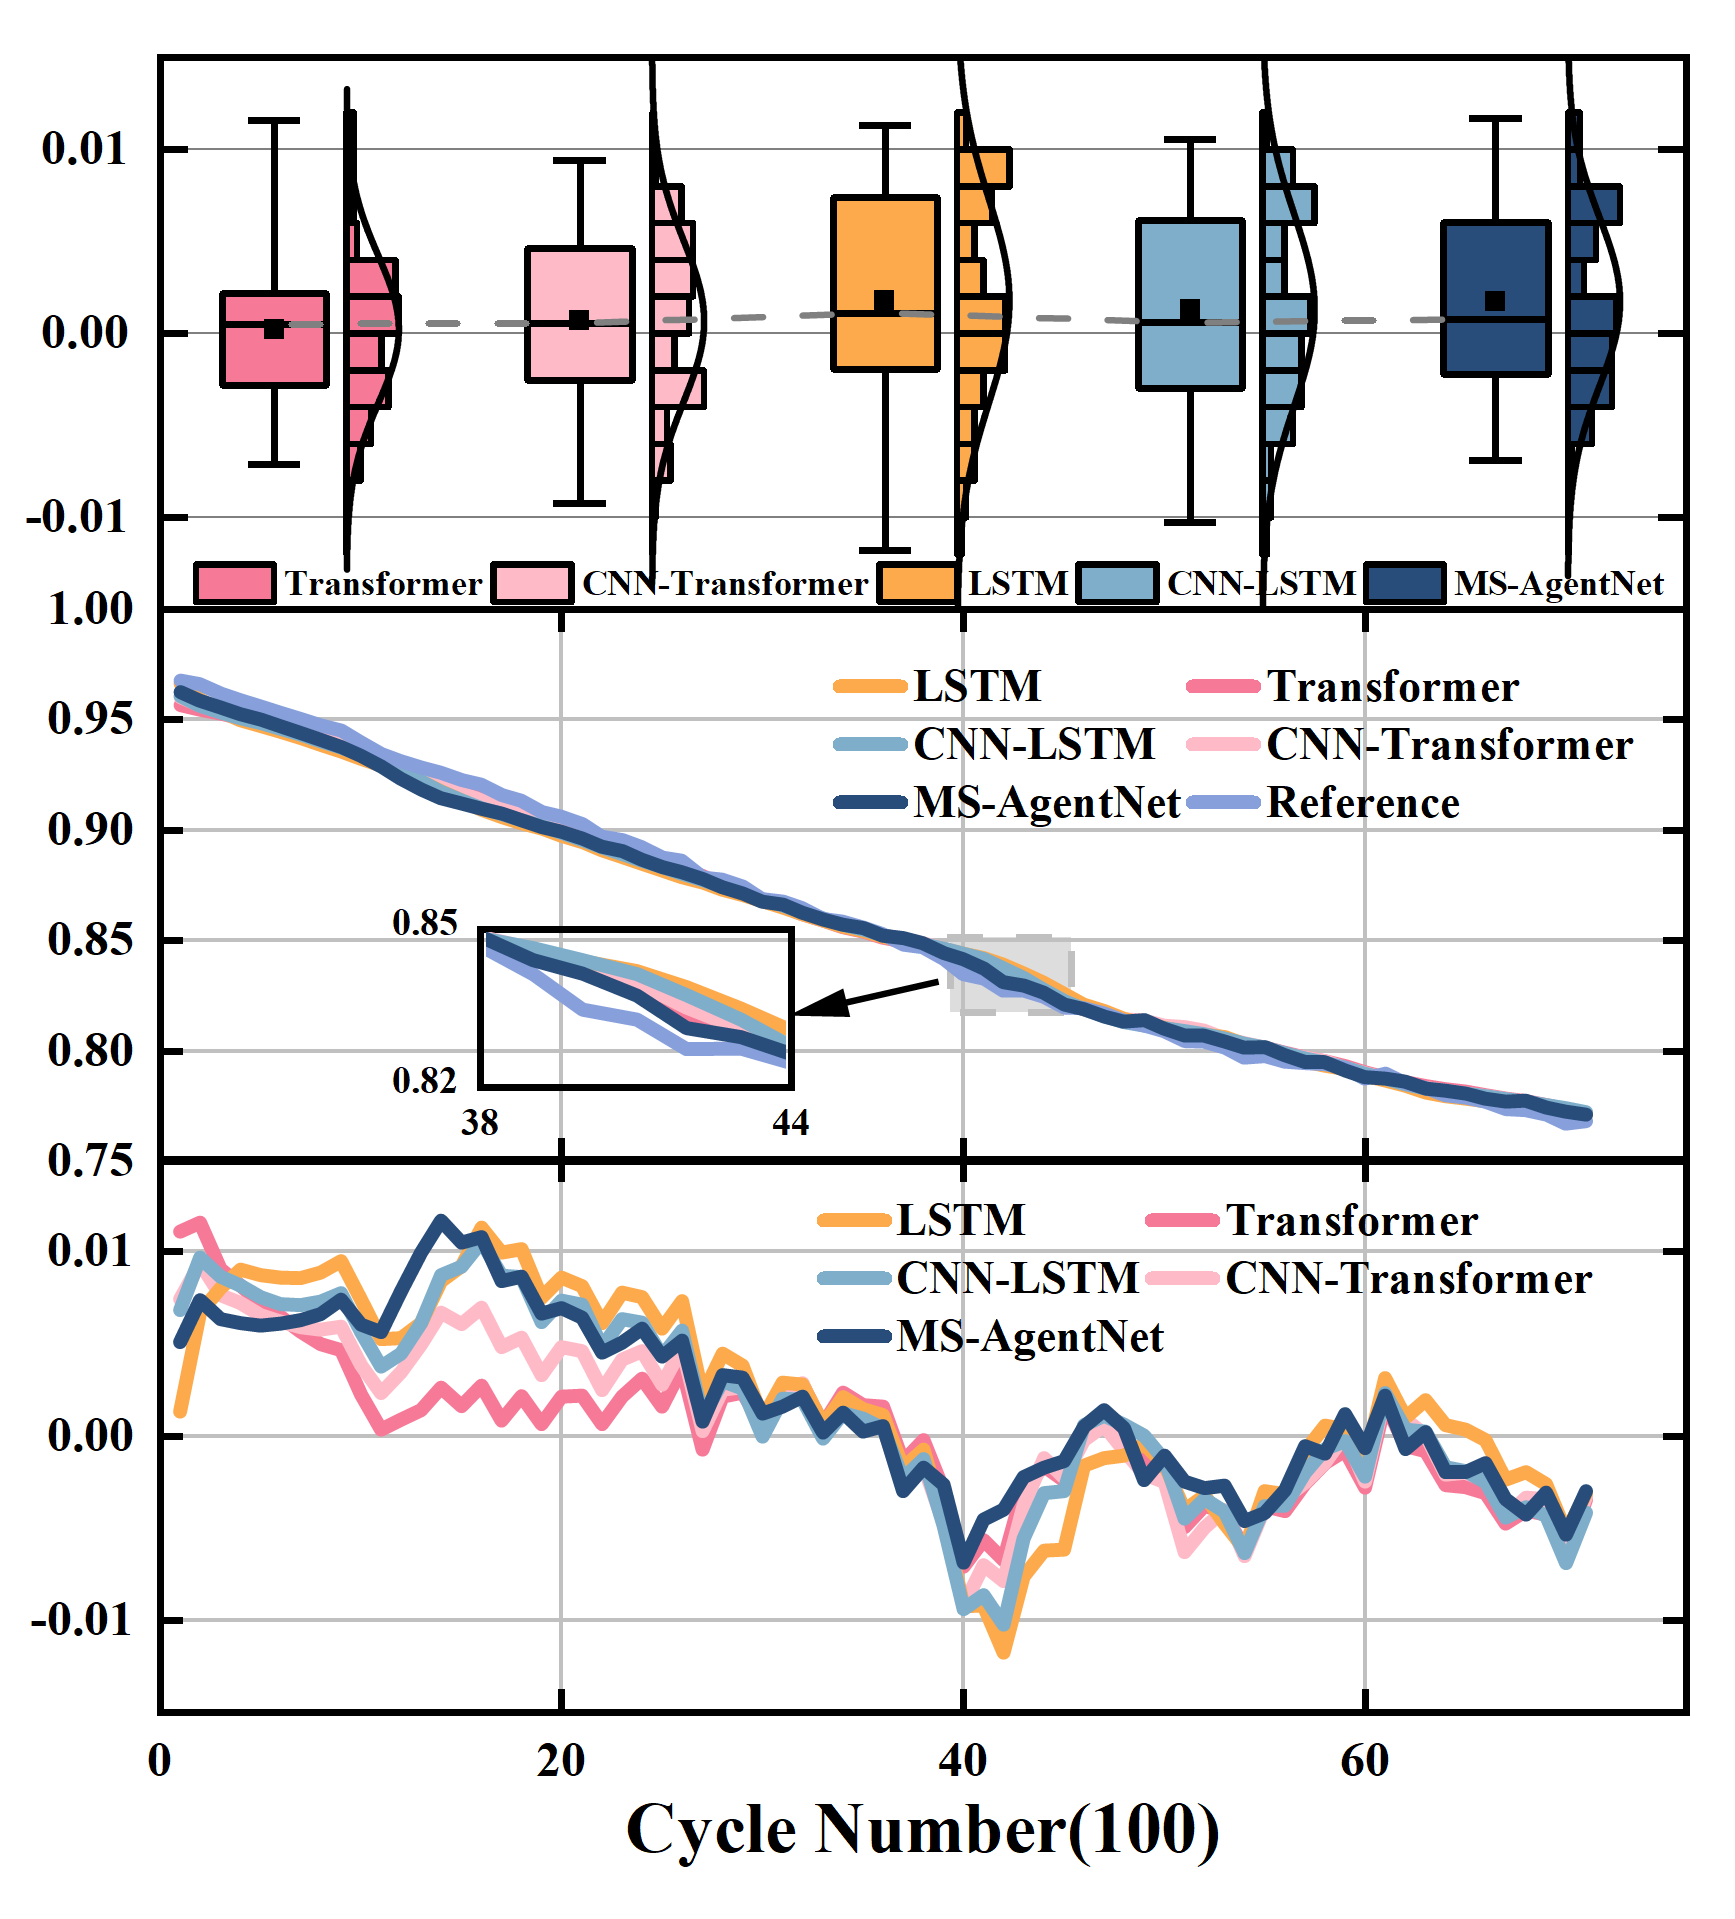
\includegraphics[width=\linewidth]{figures/Oxford/cell8.png}
\end{minipage}%
\end{minipage}%
}
\caption{SOH estimation results of different models on the Oxford dataset.}
\label{fig:4-2}
\end{figure}
